\documentclass[12pt,a4paper]{article}
\usepackage[utf8]{inputenc}
\usepackage[T1]{fontenc}
\usepackage{amsmath}
\usepackage{textcomp}

\usepackage{geometry}
\geometry{a4paper,left=25mm,right=25mm, top=2cm, bottom=2cm} 

\usepackage{graphicx} %fuer bilder

\usepackage{verbatim}



 \usepackage{mathptmx}
 \usepackage[scaled=.90]{helvet}
 \usepackage{courier}


\usepackage{listings}
\usepackage{color}
 
\definecolor{dkgreen}{rgb}{0,0.6,0}
\definecolor{gray}{rgb}{0.5,0.5,0.5}
\definecolor{mauve}{rgb}{0.58,0,0.82}

\pagestyle{empty}
\lstset{numbers=left,language=C++}
\lstset{showstringspaces=false,
basicstyle=\ttfamily\footnotesize,
breaklines=true,
tabsize=3,
commentstyle=\color{dkgreen},      % comment style
inputencoding={ansinew},
title=\lstname %zeigt titel der datei an
}

\usepackage{pdfpages}% fuer pdfs



%keine einrückungen bei absatz
\parindent 0pt

\begin{document}
\title{Übung 02}
\author{Bernhard Selymes; Reinhard Penn}
\date{April 2013}

\normalsize

%Pfad zu c++ Dateien


%Beginn des Dokuments

\newcommand{\Uebung}{Uebung02}
\newcommand{\path}{../Uebung02}

%Angabe
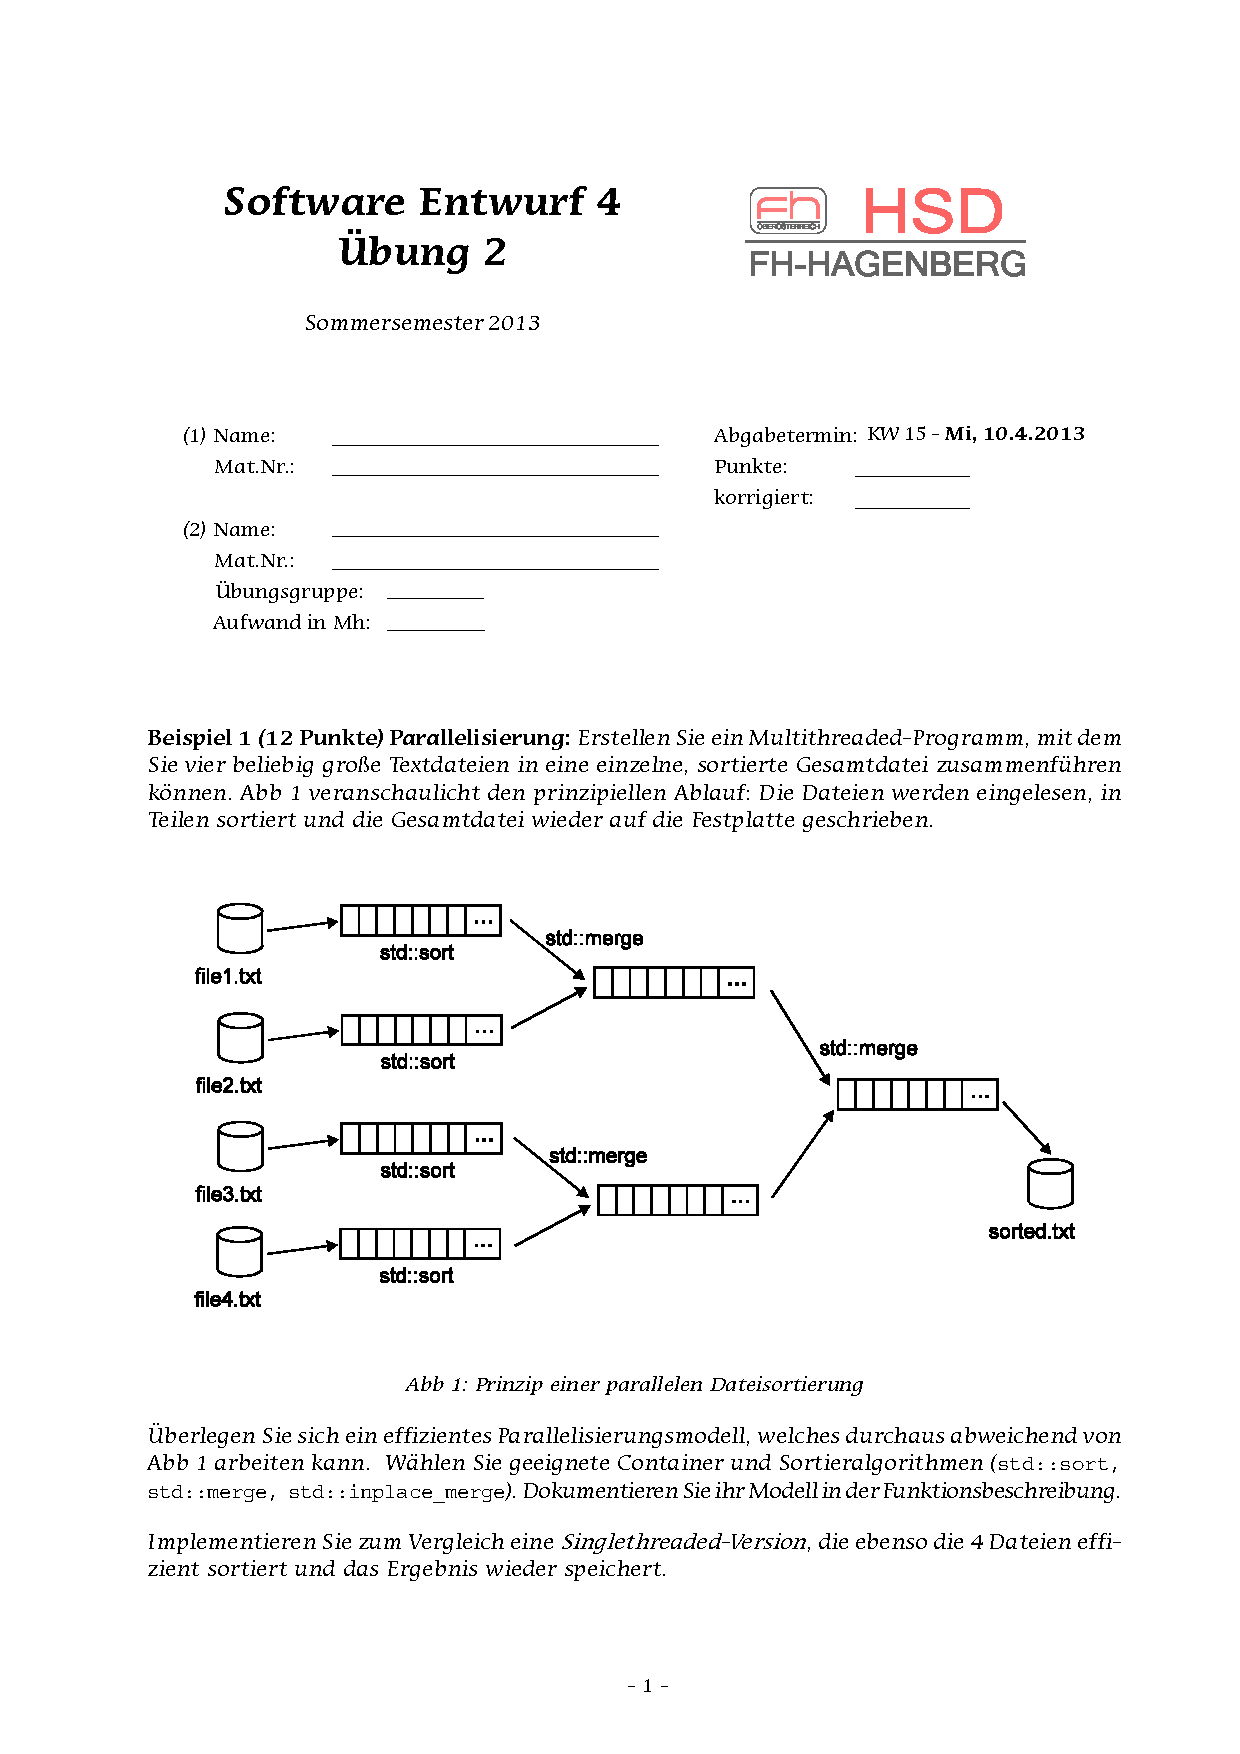
\includepdf[pages=-]{../Angabe.pdf}

\section{Beispiel 1}
\subsection{Funktionsbeschreibung}

%\newline
%\newline
%\textbf{Schnittstelle:}
%\newline
%Name: MeasureTime
%\newline
%Returnwert: double: Die Zeit die das Programm gebraucht hat.
%\newline
%Parameter: char* programName: Der Name des Programmes von dem die Zeit gemessen werden soll.


\subsection{Sourcecode}
%\lstinputlisting[language={c++}]{\path/MeasureTime/Hlp.h}
%\newpage
%\lstinputlisting[language={c++}]{\path/MeasureTime/Hlp.cpp}
%\newpage
%\lstinputlisting[language={c++}]{\path/MeasureTime/MeasureTime.h}
%\lstinputlisting[language={c++}]{\path/MeasureTime/MeasureTime.cpp}
%\newpage
%\lstinputlisting[language={c++}]{\path/MeasureTime/main.cpp}

\subsection{Testausgabe}
\begin {verbatim}

\end {verbatim}



\newpage
\section{Beispiel 2}

\subsection{Funktionsbeschreibung}

%\newline
%\newline
%\textbf{Schnittstelle:}
%\newline
%Name: CreateThreadsFib
%\newline
%Returnwert: void
%\newline
%Parameter: 
%\newline
%size\_t num: Anzahl der zu erstellenden Threads
%\newline
%size\_t fibMax: Grenzwert der Fibonacci Berechnungen


\subsection{Sourcecode}
%\lstinputlisting[language={c++}]{\path/MainThreadWorkerThread/Fibonacci.h}
%\lstinputlisting[language={c++}]{\path/MainThreadWorkerThread/Fibonacci.cpp}
%\newpage
%\lstinputlisting[language={c++}]{\path/MainThreadWorkerThread/MainThreadWorkerThread.h}
%\lstinputlisting[language={c++}]{\path/MainThreadWorkerThread/MainThreadWorkerThread.cpp}
%\newpage
%\lstinputlisting[language={c++}]{\path/MainThreadWorkerThread/main.cpp}

\subsection{Testausgabe}

\begin{verbatim}

\end{verbatim}


\end{document}
